\section{Theory} \label{sec:theory}
% Physics part
% - Composition (photometry) -> telescope optics?/instrument?/bit depth?
% - Trajectories and relative trajectory of spacecraft, especially trajectories for flybys
% - Star rendering?
% - Describe physics of SSSBs, i.e. size/shapes/surface (features/color/albedo) illumination
%
% Computer Science part
% - Physics-based rendering? -Shaders/procedural terrain generation
% - Compression
% - Reconstruction (SfM), relates to camera physics. Generally Computer Vision topic.
% - Image processing Gaussian filtering, downscale local means
% - Logic for choosing number of reconstructed points as quality measure
%
% Space
% - Small Spacecrafts -> small data budgets?
%
% Max Science?
%
% Concepts to describe???


\subsection{Small Solar System Bodies}
The \gls{iau} defines an \gls{sssb} as any object in the Solar System, that is not a planet, dwarf planet or satellite~\cite{iau_sssb}. Within this work, the term \gls{sssb} mostly refers to asteroids and comets.

In a classical definition, asteroids and comets were two distinct \glspl{sssb} classes based on observational, physical and dynamical properties. However, the discovery of active asteroids and dormant comets began to blur these definitions. Since many observed objects cannot be strictly classified into the classical categories anymore, it is becoming more common to describe these objects as part of a asteroid-comet continuum with asteroids and comets at the ends of the continuum~\cite{Hsieh2017Asteroid-cometSystem}.

Despite the shift towards a continuum definition, we refer to non-active objects as asteroid and active objects as comets within this work in cases where it is necessary to distinguish between these types of objects. Therefore, a description for the classical definition of asteroids and comets is provided.

\subsubsection{Asteroids}
Asteroids are rocky bodies that mostly reside in an orbit between Mars and Jupiter, i.e. the asteroid main belt. The terms asteroid and minor planet are often used interchangeably. About \SI{930000}{} asteroids are known of which only about \SI{540000}{} are numbered. Since most asteroids are only observed remotely, only their ephemeris and absolute magnitude ($\approx \SI{925000}{}$) is observed. Approximately, only \SI{136000}{} asteroids have a known diameter~\cite{JPLEngine}. However, a few asteroids also have physical parameters like albedo ($\approx \SI{135000}{}$) , rotation period ($\approx \SI{19000}{}$) , spectral type ($\approx \SI{2000}{}$) and the standard gravitational parameter ($\approx \SI{10}{}$)~\cite{JPLEngine}.

The asteroids Bennu and Ryugu are described as rubble piles due to the low density~\cite{Chesley2014OrbitBennu, Watanabe2019Hayabusa2Pile}. The rubble pile concept refers to objects which aggregated boulders by gravity giving them a low bulk density because of many void spaces in there internal structure~\cite{Richardson2002GravitationalEvolution}.

\subsubsection{Comets}
Comets are small icy bodies that mostly reside farther away from the Sun than asteroids. Inside the heliosphere, the source of comets is the Kuiper belt while comets from outside the heliosphere are thought to originate in the Oort cloud. On long timescales, comets are perturbed by the gravity of other objects which alters their orbits and moves them closer to the Sun. While being close to the Sun, volatiles begin to evaporate. This creates the well known coma around the nucleus of a comet. In most cases the coma is several orders of magnitudes larger than the nucleus, the nucleus is on the order of a few kilometres while the coma can be on the order of hundreds of thousands of kilometres. Additionally, two tails are formed, a gas and a dust tail. The gas tail is formed from coma particles that move away from the nucleus and are then carried away by the magnetic field carried by the solar wind. On the other hand, the dust tail is formed from small dust particles in the coma which are carried away from the nucleus by the solar radiation pressure. Larger dust particles remain along a comets trajectory forming part of the meteoroid environment~\cite{Soja2019IMEM2:System, a2017comets, Comets}.

The physical parameters of comets are not well known, since they are small and it is difficult to image the nucleus when they come closer to the Sun since the nucleus is surrounded by the coma. Approximately \SI{3500}{} comets are known of which only about \SI{400}{} are numbered~\cite{JPLEngine}. While the ephemeris ($\approx \SI{1700}{}$) and magnitude ($\approx \SI{1300}{}$) are known for many comets, for only a few comets physical properties like the diameter ($\approx \SI{100}{}$) or the rotation period ($\approx \SI{20}{}$) are known~\cite{JPLEngine}.

It is not clear whether comets are generally similar to rubble piles or rather consolidated, monolithic bodies. It is assumed that most bodies in the range of \SI{200}{\meter} to \SI{10}{\kilo\meter} are rubble piles~\cite{Walsh2018RubbleAsteroids}. However, density measurements and surface features of \gls{67p} are not conclusive so far~\cite{Weissman2020OriginNuclei}. 

\subsubsection{Orbit Mechanics} \label{sec:orbit_mechanics}
All objects in space move on trajectories, or orbits if closed, following the Kepler equations. Trajectories are commonly defined using six orbital elements.
Semi-major axis $a$, eccentricity $e$, inclination $i$, right ascension of ascending node $\Omega$, argument of periapsis $\omega$ and the true anomaly $\nu$ or mean anomaly $M$ at a given epoch. This parameterisation is also called modified Keplerian elements~\cite{Hintz2015FundamentalsAstrodynamics}.

Figure~\ref{fig:kepler_elements} shows the geometric relations of the angular Elements.

\begin{figure}[htb]
    \centering
    \begin{subfigure}[b]{0.47\textwidth}
        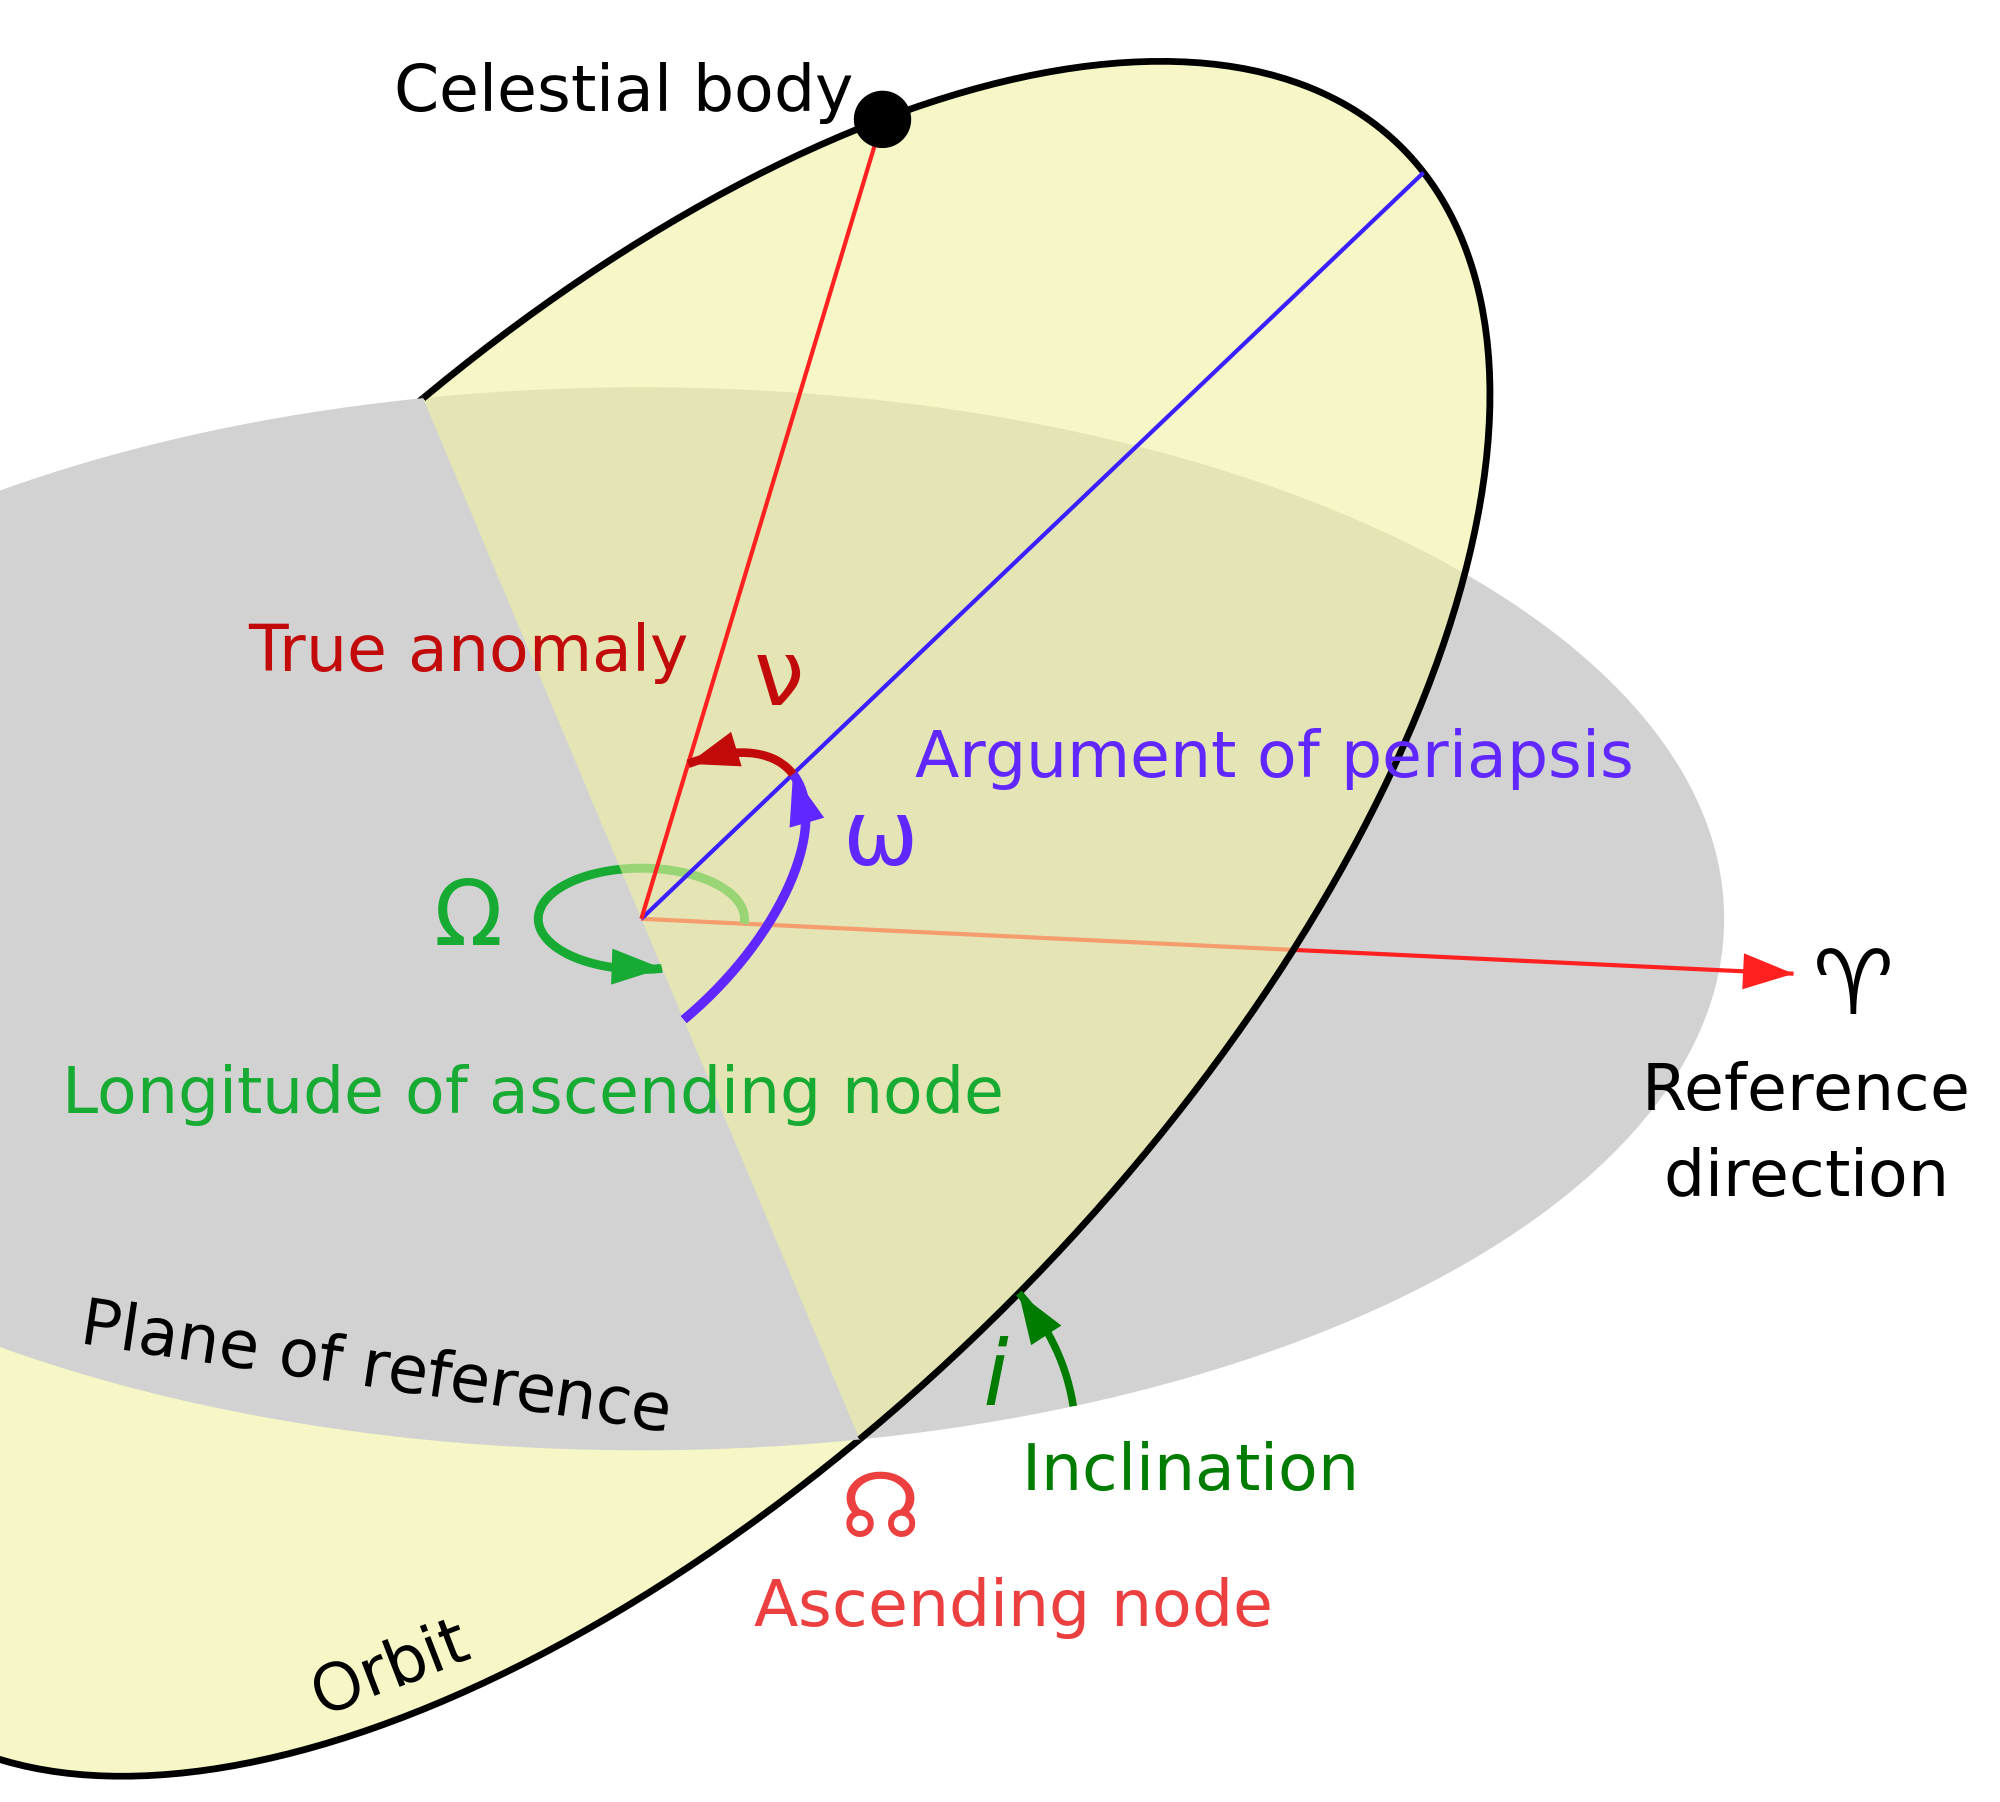
\includegraphics[width=.8\textwidth]{doc/thesis/0_figures/Orbit_elements.png}
        \caption{}
        \label{fig:kepler_elements}
    \end{subfigure}
    \begin{subfigure}[b]{0.47\textwidth}
        \centering
        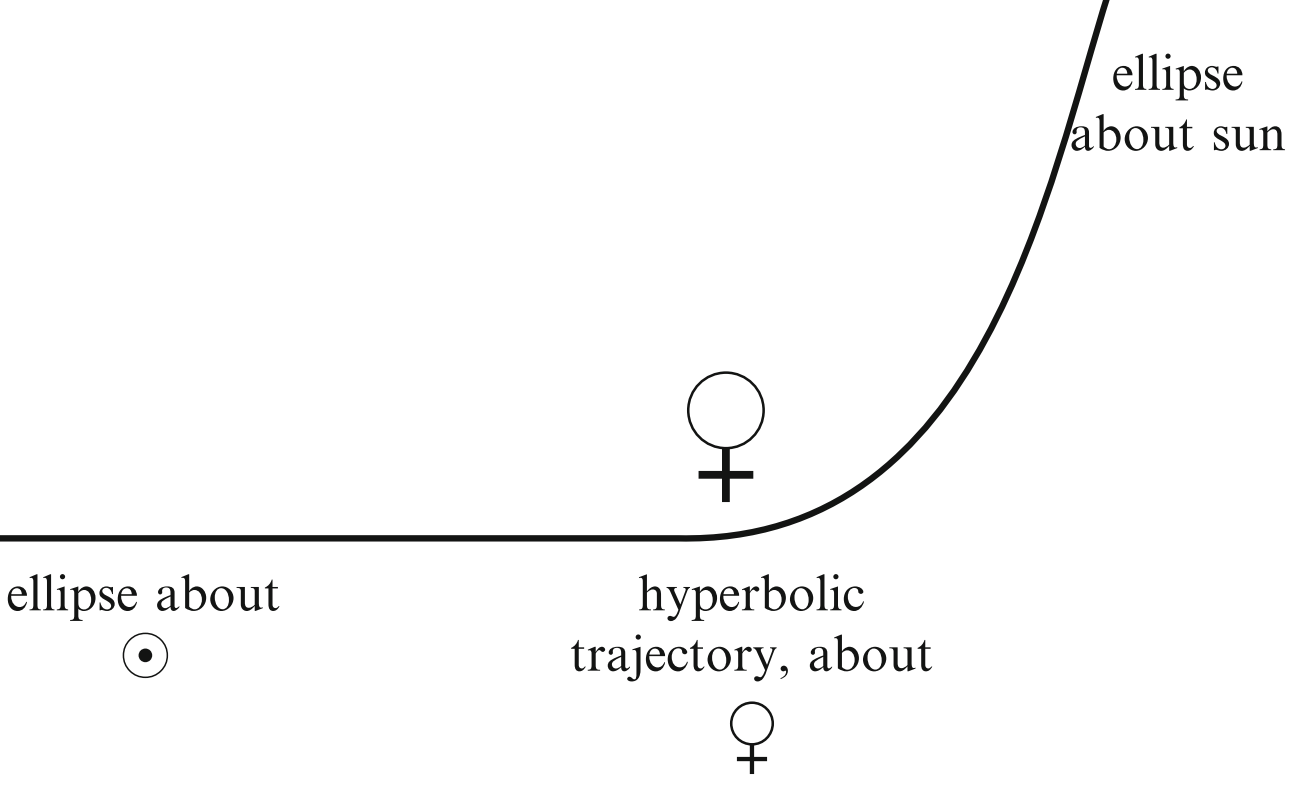
\includegraphics[width=\textwidth]{doc/thesis/0_figures/Hyperbolic_trajectory.png}
        \caption{}
        \label{fig:hyperbolic_orbit}
    \end{subfigure}
    \label{fig:astrodynamics}
    \caption{Important astrodynamic definitions and relations. (a) Modified Keplerian elements \cite{Commons2019File:Orbit1.svgRepository}. (b) A closed orbit around the Sun (\astrosun) becomes a hyperbolic trajectory about another body, Venus (\venus) in this example \cite{Hintz2015FundamentalsAstrodynamics}.}
\end{figure}

Flyby scenarios in the Solar System are often closed orbits around the Sun, i.e. $e_{\astrosun} < 1$ while they are hyperbolic trajectories in the reference frame of the target, i.e. $e_{\venus} > 1$. An example is given in Figure~\ref{fig:hyperbolic_orbit}. A high relative velocity and the small gravitational force exerted by a \gls{sssb} result in a trajectory closer to a straight line than the bend trajectory presented in Figure~\ref{fig:hyperbolic_orbit}. 

Most asteroids move on orbits with low eccentricity while comets often have high eccentricities. This stems from their origin, while asteroids mostly origin from the main belt which is nearly circular region, comets enter the inner Solar System from far out, i.e. there aphelion is still far from the Sun resulting in high eccentricities.

\subsection{Rendering}
Rendering is the process of creating \gls{2d} images from \gls{3d} objects. For rendering, a virtual world is created where \gls{3d} models reside. Light sources and cameras produce artificial illumination and define which part of the world is being captured. A rendering engine calculates the pixel values to generate the final image based on energy conservation by using the rendering equation~\cite{Kajiya1986TheEquation}.

\subsubsection{Path Tracing}
Path tracing is a special form of ray tracing. Ray tracing is a rendering technique where the path of light rays is traced to generate pixels while simulating effects of encounters with objects. In path tracing not individual light rays are followed which then branch into an exponentially growing number of rays when being reflected or refracted but only a single path is followed, cutting computation time dramatically in cases with a lot of reflection, refraction and shadow rays per pixel~\cite{Kajiya1986TheEquation}. Ray tracing can simulate different effects, such as reflection, refraction, scattering and dispersion. While producing a high degree of realism in images, the computational costs are high as well. There are four types of rays: camera rays, reflection rays, transmission rays and shadow rays. Reflection and transmissions can be further categorised as either diffuse, glossy or singular. Ray tracing is a popular rendering technique where a high degree of realism is necessary since it is a realistic simulation of light transport.

\subsubsection{3D Models and Shaders}
A \gls{3d} model is a set of points in \gls{3d} space. The most common type of \gls{3d} models are polygonal meshes. Polygonal meshes are shell models that consist of polygons. A vertex is a corner of a polygon, i.e. every triangle has three vertices and every tetrahedron has four vertices. A face refers to the surfaces that make up a \gls{3d} model. Depending on the rendering environment, models are more or less sophisticated and their surface can have different properties such as reflection, refraction and transmission.

A shader is used to calculate effects during the rendering process. Shaders are meant to provide a flexible method to influence the rendering outcome during the rendering process. Shaders can be used to change the positions of vertices, colours, lighting and surface properties by using equations. Through the interplay of these properties, it is possible to generate complex surface structure and texture procedurally generating details as needed. While shaders are not restricted to be executed on a \gls{gpu}, it is commonly done since a \gls{gpu}'s hardware is well suited for this task.
Common shaders that influence the surface of an object are using a \gls{bsdf}. A \gls{bsdf} is a mathematical function that describes light scattering behaviour of the surface of a \gls{3d} model. There are several classes of \glspl{bsdf} such as diffuse, glossy, refraction and transparent shaders that create the respective effect based on a small set of input parameters.

\subsubsection{Field of View}
The \gls{fov} defines the extent of the \gls{3d} scene that is visible from the camera. From geometric considerations, vectors that point to the edges of the \gls{fov} can be constructed using
\begin{align}
    e_{i} = v_d \pm \frac{v_j \times s_k}{2 \times f}, \label{eq:fov_edge}
\end{align}
where $e_{i}$ is a vector for the $i^{th}$ edge of the \gls{fov}, $v_d$ is the direction vector of the camera, $v_j$ is the vector pointing right or up in the \gls{fov} plane, $s_k$ is the camera sensor width or height and $f$ is the focal length. The left and right edge vectors, $e_{left}$ and $e_{right}$, are calculated with the vector $v_r$ pointing right in the \gls{fov} plane and the sensor width $s_w$. The upper and lower edge vectors, $e_{upper}$ and $e_{lower}$  are calculated with the vector $v_r$ pointing up in the \gls{fov} plane and the sensor height $s_h$.

In addition to the extent of the \gls{fov} within the image plane, rendering requires the view to be clipped to a minimum and maximum distance to define which objects appear in a rendered scene. The clipping is necessary to limit the required computational power for rendering. 

\subsubsection{Photometric calibration} \label{sec:photo_cal}
Photometric calibration is the process of correcting raw images from a sensor to a common level of brightness. Differences might come from different exposure times, gains or cameras. Photometric calibration uses a photometric systems, such as the \gls{ubv}, which are reference systems with which star magnitude measurements can be compared for a given band of the system~\cite{Bessell1979UBVRIPhotometry}.

The apparent magnitude of a star is converted into photon flux density relative to magnitude 0 by using,
\begin{align}
    F = 10^{-0.4 \times m}, \label{eq:mag_flux}
\end{align}
where $m$ is the apparent star magnitude. 
Given the apparent magnitude of a specific band, the photon flux density of a reference object can be calculated using
\begin{align}
    F = F_0 \times \frac{d\lambda}{\lambda} \times 10^{-0.4 \times m}, \label{eq:comp_flux_0mag}
\end{align}
with $F_0$ being the flux at magnitude 0, $\frac{d\lambda}{\lambda}$ is a factor that depends on the band, and $m$ is the object's magnitude. The required constants to calculate the photon flux of an object from its magnitude in a given band are given in Table~\ref{tab:ubv_constants}.

\begin{table}[htb]
    \centering
    \caption{Constants for calculating photon fluxes using the \gls{ubv}~\cite{Bessell1979UBVRIPhotometry}.}
    \label{tab:ubv_constants}
    \begin{tabular}{l|l|l|l}
        \textbf{Band} & \textbf{Centre Wavelength [\SI{}{\nano\meter}]} & \textbf{$F_0$ [\SI{1e-26}{\watt\per\square\meter\per\hertz}]} & \textbf{$\frac{d\lambda}{\lambda}$}[~] \\ \hline
        U             & 0.36                       & 1810        & 0.15             \\
        B             & 0.44                       & 4260        & 0.22             \\
        V             & 0.55                       & 3640        & 0.16            
    \end{tabular}
\end{table}

The next step of photometric calibration is to calculate the reference photon flux for one pixel of the \gls{ccd} $F_{ref}$ using
\begin{align}
    F_{ref} = F \times \frac{A \times A_{pixel}}{f^2 \times \pi}, \label{eq:comp_flux_pix}
\end{align}
where $F$ is the photon flux density, $A$ is the aperture area, $A_{pixel}$ is the area of a pixel and $f$ is the focal length of the instrument.

In the last step, the calibration factor is calculated. It is defined as
\begin{align}
    f_c = \frac{F_{ref} \times \alpha}{I_{ref}}, \label{eq:comp_cal_fac}
\end{align}
where $F_{ref}$ is the reference flux, $\alpha$ is the geometric albedo and $I_{ref}$ is the reference intensity. Multiplying the image with $f_c$ produces the calibrated image.

The effect of photometric calibration is delineated in Figure~\ref{fig:t_photometry}. Photometric calibration corrects the brightness difference of a set of images towards a common brightness level.
\begin{figure}[htb]
    \centering
    \begin{subfigure}[b]{0.25\textwidth}
        \centering
        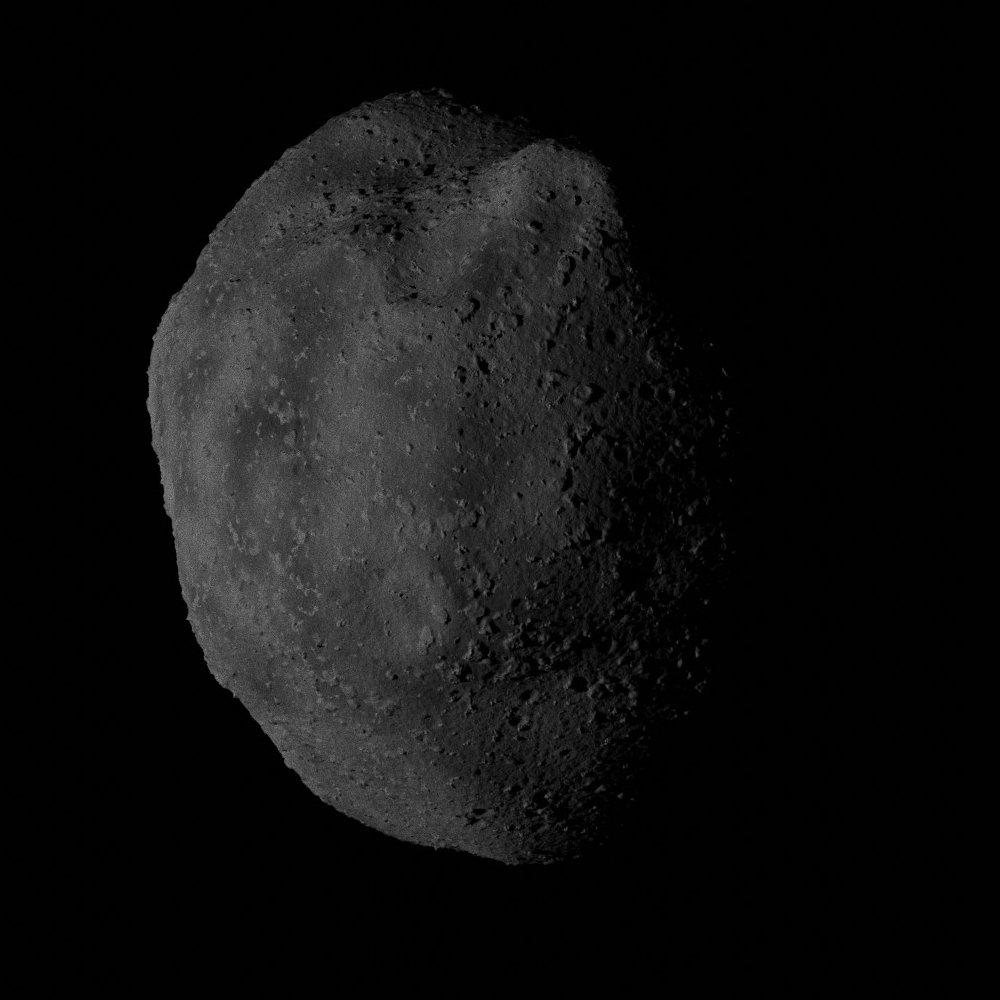
\includegraphics[width=\textwidth]{doc/thesis/0_figures/rendering_lighting/Before_1.png}
        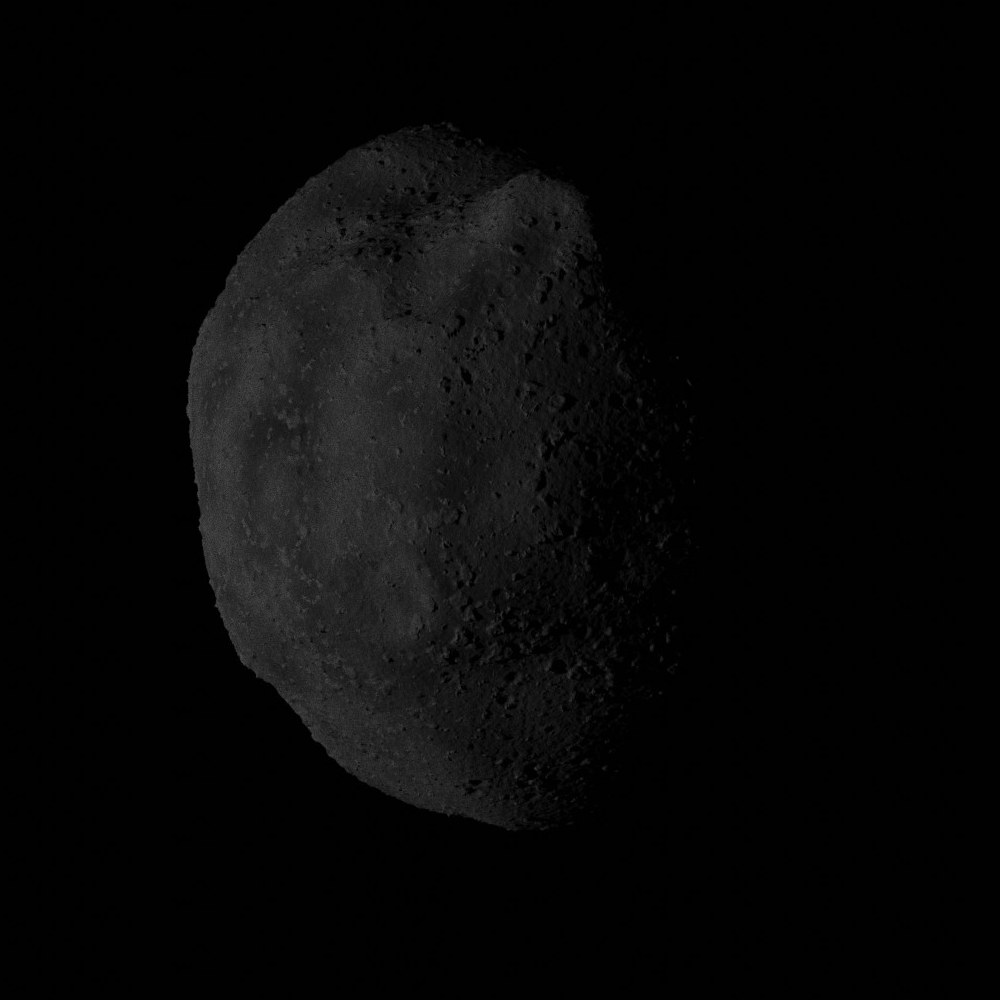
\includegraphics[width=\textwidth]{doc/thesis/0_figures/rendering_lighting/Before_2.png}
        \caption{}
        \label{fig:t_photometry_1}
    \end{subfigure}
    \begin{subfigure}[b]{0.25\textwidth}
        \centering
        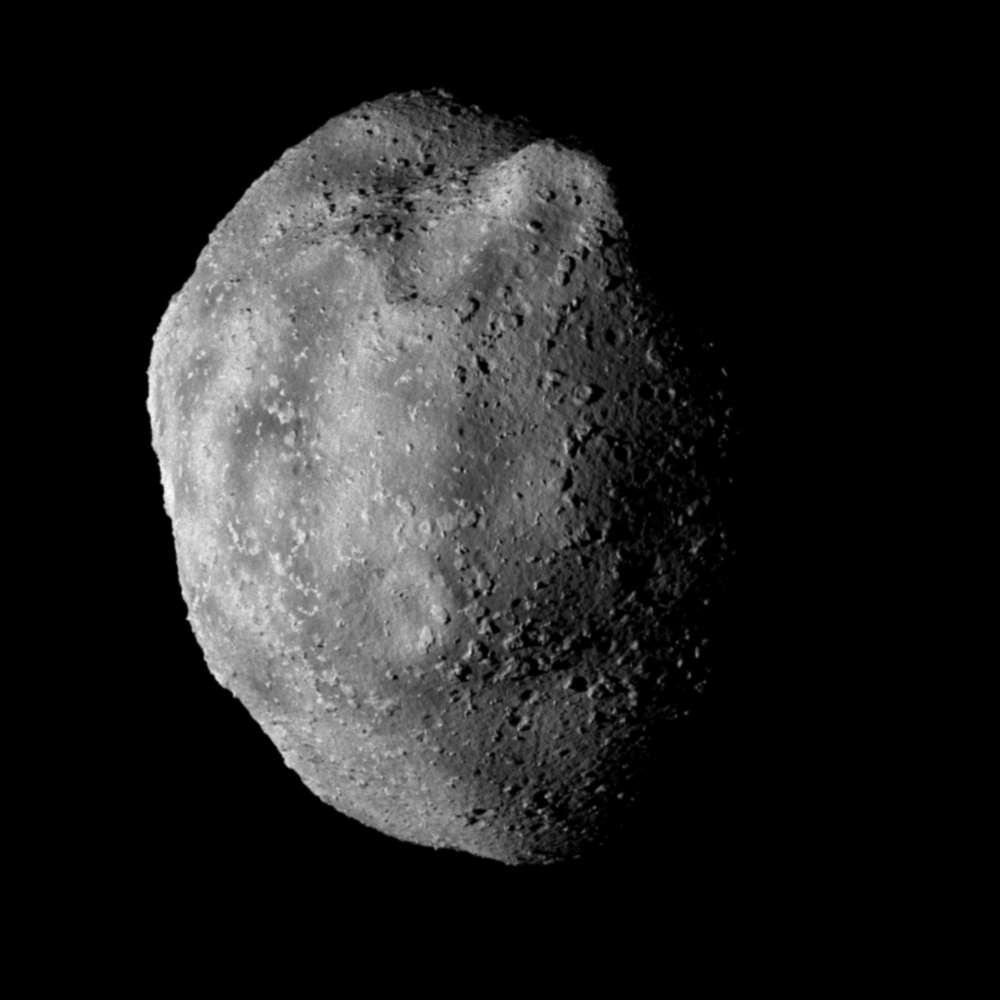
\includegraphics[width=\textwidth]{doc/thesis/0_figures/rendering_lighting/After_1.png}
        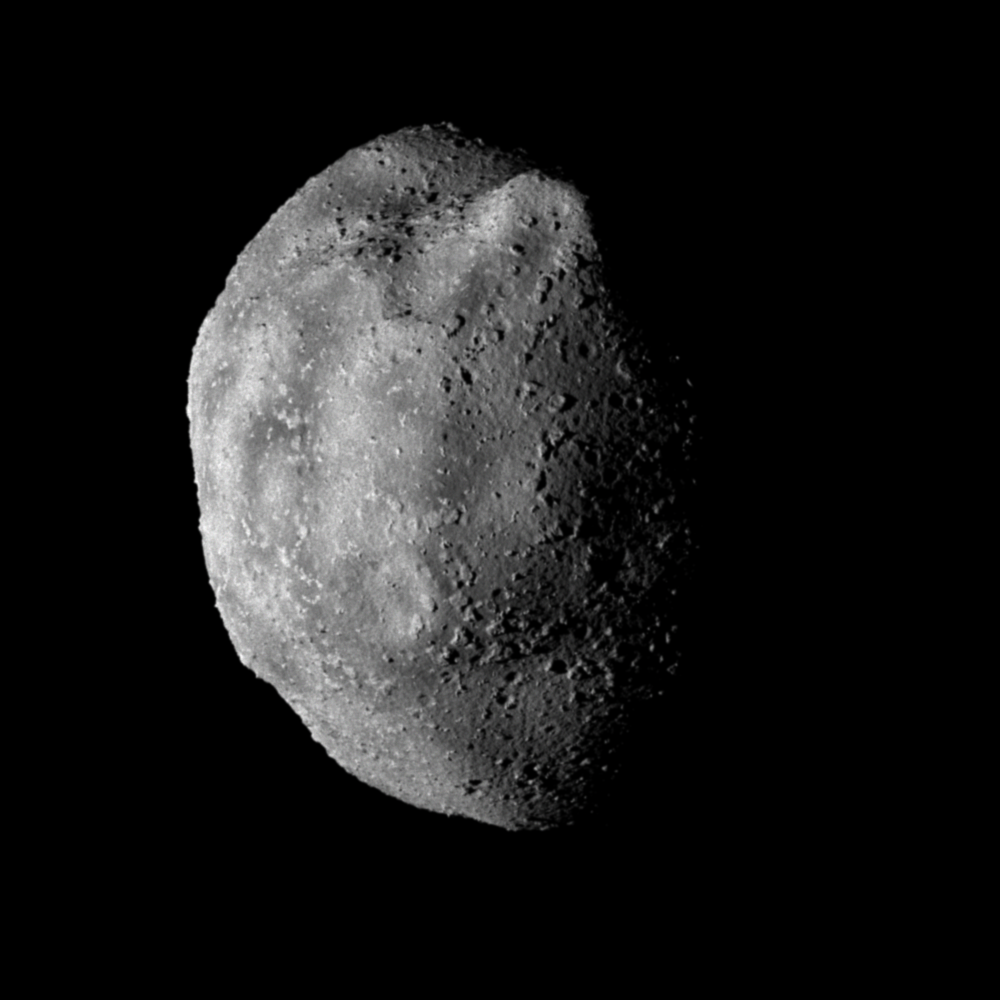
\includegraphics[width=\textwidth]{doc/thesis/0_figures/rendering_lighting/After_2.png}
        \caption{}
        \label{fig:t_photometry_3}
    \end{subfigure}
    \caption{Two consecutive images (a) before and (b) after photometric calibration which eliminated the brightness difference of the original images.}
    \label{fig:t_photometry}
\end{figure}

\subsection{Computer Vision} \label{sec:t_cv}
\Gls{cv} is the science of extracting information from digital photos and videos by mimicking the human vision system using a computer. \Gls{cv} encompasses a wide field of activities, from image formation, processing, detecting and matching features, image segmentation and \gls{3d} reconstruction~\cite{szeliski2010computer}. \Gls{cv} is the computer based variant of photogrammetry which is tasked with obtaining information about physical objects and the environment from photographic images~\cite{Kasser2002DigitalPhotogrammetry}. The most common approach for \gls{3d} reconstruction is stereo-photogrammetry, also referred to as computer stereo vision. Stereo-photogrammetry applies the binocular vision principle of the human vision system to obtain structural information from images~\cite{do2019review}. Since most, if not all, deep space missions have a visual imager instrument on-board, \gls{cv} provides a useful framework to obtain the \gls{3d} structure of an observation target. A similar problem is the \gls{sfm} approach where the motion of the camera creates the different perspective.

\subsubsection{Pinhole Camera Model}
All \gls{cv} problems require a model of a camera. The most commonly used model in \gls{cv} is the pinhole camera. Figure~\ref{fig:pinhole_cam} gives a simple overview of the important parts of the pinhole model.

\begin{figure}[htb]
    \centering
    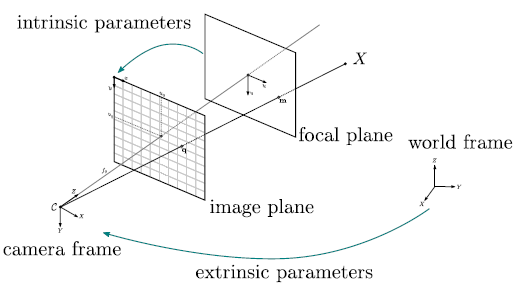
\includegraphics[width=\textwidth]{doc/thesis/0_figures/sfm/pinholeCamera.png}
    \caption{Overview of the components of the pinhole camera model~\cite{openMVG}. The camera intrinsic parameters model the optics, the extrinsic parameters model the camera position and orientation. The image plane is the plane of the \gls{ccd} and the focal plane is the plane where the focus of the optical system is.}
    \label{fig:pinhole_cam}
\end{figure} 

The pinhole camera model can be described using the $3\times4$ camera matrix $\textbf{K}$ defined as
\begin{align}
    \textbf{K} = \begin{bmatrix}
        f\times k_u & 0           & c_u \\
        0           & f\times k_v & c_v \\
        0           & 0           & 1   \\
    \end{bmatrix} 
    \begin{bmatrix}
        \textbf{R} & t
    \end{bmatrix}, \label{eq:camera_m}
\end{align}
where $f$ is the distance between the focal plane and the image plane, $k_u$ and $k_v$ to are scaling factors, $c_u$ and $c_v$ are the coordinates of the principle point on the image plane, $R$ is a $3\times3$ rotation matrix and $t$ being a $3\times1$ translation vector. The first matrix of $\textbf{K}$ reflects the camera intrinsic parameters while the second matrix describes the extrinsic parameters.
More sophisticated pinhole camera models also include distortions. These can include one or more factors for radial and tangential distortions. A special case it the Brown T2 model which includes three radial and two tangential distortion factors.

The conversion between object coordinates and pixel coordinates is obtained from geometric considerations of the pinhole camera model shown in Figure~\ref{fig:pinhole_cam} and is defined as
\begin{align}
    x_{pix} = 2 \times \frac{f}{s_w} \times \frac{\hat{v}_r \cdot p}{\hat{v}_d \cdot p + 1} \times \frac{(r_x - 1)}{2}, \label{eq:pix_conversion} 
\end{align}
%x_pix = ss * (f_over_w_ccd_2 * np.dot(right_norm, vec) / np.dot(direction, vec) + 1.) * (res_x - 1) / 2.
where $x_{pix}$ is the x-coordinate of the pixel in the image frame, $f$ is the focal length, $s_w$ is the sensor width, $v_r$ is the unit vector pointing right in the image plane, $p$ is the Cartesian coordinate vector of a star, $v_d$ is the direction vector of the \gls{fov} and $r_x$ is the number of pixels in x-direction. Similarly, the conversion for y-coordinate of a pixel $y_{pix}$ is obtained by replacing the sensor width $s_w$ with the sensor height $s_h$, $v_r$ by the unit vector $v_u$ pointing up in the image plane and the number of pixels in x-direction $r_x$ by the number of pixels in the y-direction $r_y$. The vectors $v_r$ and $v_u$ are calculated by subtracting $v_d$ from the field of view edge vectors $e_{right}$ and $e_{upper}$ as defined in Equation \ref{eq:fov_edge}.

\subsubsection{Structure-from-Motion}
\Gls{sfm} can be considered the inverse process to rendering, i.e. creating \gls{3d} models from \gls{2d} images. \gls{sfm} uses multiple views of the same object from different camera positions to reconstruct its geometry. \Gls{sfm} encompasses the recovery of the \gls{3d} structure of an object as well as camera poses~\cite{szeliski2010computer}. Depth information is obtained through the motion parallax created by the moving camera. Generic steps of an \gls{sfm} processing pipeline are shown in Figure~\ref{fig:sfm_steps}.

\begin{figure}[htb]
    \centering
    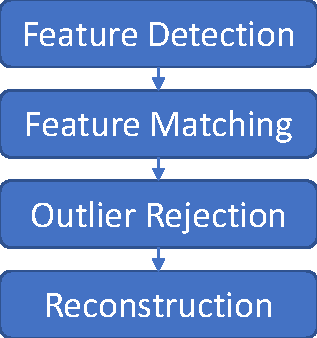
\includegraphics[width=.25\textwidth]{doc/thesis/0_figures/sfm/SfM.pdf}
    \caption{Generic steps of a \gls{sfm} processing pipeline.}
    \label{fig:sfm_steps}
\end{figure}

Figure \ref{fig:sfm_geometry} shows a generic observation geometry. A camera at different positions with feature points on their respective image plane and the relation between this feature point and the object point are depicted. 

\begin{figure}[htb]
    \centering
    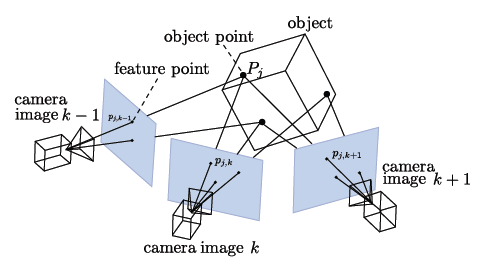
\includegraphics[width=\textwidth]{doc/thesis/0_figures/sfm/sfm_geometry.png}
    \caption{Generic observation geometry in a \gls{sfm} problem~\cite{andrews2019asteroid}. The \gls{3d} structure can be reconstructed from several point observations and intrinsic camera parameters.}
    \label{fig:sfm_geometry}
\end{figure}

To reconstruct \gls{3d} points from an image series, correspondence between images needs to be found. This is achieved by detecting features in an image that can be detected and matched in multiple images. A feature can be described as a local, meaningful and detectable part of an image. Features are being used because of their high information content. Features can be image regions of sudden change, shape features or texture contours. Commonly detected features are corners, edges, junctions, blobs and lines~\cite{Tareen2018ABRISK}. These features are described using feature descriptors which assign a distinct identity to the described feature for later matching. A range of different feature detection algorithms  exist, sometimes with a ready to use algorithm. While most feature detectors are combined with a distinct feature descriptor, it is possible to interchange these. Feature detectors are tasked with detecting feature-points in an image. Feature points are also referred to as key-points or interest-points. A common requirement for good feature descriptors and detectors is that both should be scaling, rotation and affine invariant. The most commonly known feature detectors and descriptor pairs are \gls{sift}, \gls{surf}. \gls{orb}, KAZE and \gls{akaze}~\cite{Tareen2018ABRISK}.
% Add SIFT description?
After features are detected and described in all images, these features need to be matched, i.e. an algorithm identifies the same feature in multiple images. Depending on the descriptor, either an L1 or L2 norm for a scalar descriptor or the hamming distance for binary descriptor are used. Feature matching can be carried out between image pairs or between a longer series of images. Different geometries can be described using different mappings. The homography matrix $\textbf{H}$ describes mapping of coordinates from two different views and is defined as
\begin{align}
    x'_i = \textbf{H}x_i, \label{eq:homography_m}
\end{align}
where $x'_i$ are the coordinates of point $i$ in the second image, $x_i$ are the coordinates of point $i$ in the first image and $\textbf{H}$ is the homography matrix. However, $\textbf{H}$ describes only a purely rotating or moving camera capturing a planar scene~\cite{schonberger2016structure}.
The fundamental matrix $\textbf{F}$ describes the relation between two images of the same scene for a moving camera. It relates points of uncalibrated images and is defined as
\begin{align}
    {x'_i}^{T}\textbf{F}x_i = 0, \label{eq:fundamental_m}
\end{align}
where $x'_i$ are the coordinates of point $i$ in the second image, $x_i$ are the coordinates of point $i$ in the first image and $\textbf{F}$ is the fundamental matrix. The epipolar line
\begin{align}
    l'_i = \textbf{F}x_i, \label{eq:epipolar_l}
\end{align}
where $l'_i$ is the epipolar line, $\textbf{F}$ is the fundamental matrix and $x_i$ are the coordinates of a point in the first image. This line constitutes all possible positions of point $x'_i$.

If additionally, the camera intrinsics are taken into account, the fundamental matrix becomes the essential matrix $\textbf{E}$ which is defined as
\begin{align}
    \textbf{E} = \textbf{K}'^{T}\textbf{F}\textbf{K}, \label{eq:essential_m}
\end{align}
with $\textbf{E}$ being the essential matrix, $\textbf{K}'$ being the camera matrix of the second view, $\textbf{F}$ being the fundamental matrix as defined in Eq. \ref{eq:fundamental_m} and $\textbf{K}$ being the camera matrix of the first view. Therefore, the essential matrix is intended for use in conjunction with calibrated images where the camera intrinsics are available.
If sufficient number of points are being mapped correctly using one of the transformation from Equations \ref{eq:homography_m}, \ref{eq:fundamental_m} or \ref{eq:essential_m}, the points are geometrically verified.

However after geometric verification, there might still be outliers. Therefore, outlier rejection is performed as an additional step to remove incorrect matches. Several algorithms such as \gls{ransac}~\cite{Fischler1981RandomCartography}, \gls{acransac}~\cite{moisan2012automatic}, \gls{msac}~\cite{wang2009generalized} and \gls{prosac}~\cite{Chum2005MatchingConsensus} are used for outlier removal. All of these algorithms aim at robustly estimate the correct model and remove outliers. The result of this step is the view graph that relates the different views to each other with images as nodes and pairs as edges~\cite{schonberger2016structure}.

Using the view graph as an input, the reconstruction process produces a \gls{3d} point cloud. A point cloud is a set of independent points with coordinates in \gls{3d} space. There are two principle methods for reconstruction, incremental and global. In case the image set is unordered, the more common approach is to use the incremental approach~\cite{schonberger2016structure}.

Incremental reconstruction starts with an initial pair of views. Selecting this initial pair is a critical step as the reconstruction algorithm might not converge after using a bad initial pair. Typically, starting with a scene with many overlapping camera views constitutes a robust initialisation and results in higher accuracy because of the redundant information from many images~\cite{schonberger2016structure}.
Consequently, additional images are registered to the current model based on corresponding features which can be used to triangulate additional points in already registered images. This step can includes estimating the pose of a camera and also the camera intrinsic parameters for uncalibrated images. Triangulation is an essential step of making \gls{sfm} robust by adding redundant information about existing points in a model and adding additional points to increase the coverage of the model~\cite{schonberger2016structure}. To help these algorithms to converge, it is possible to provide initial pose estimates, so called priors.
Image registration and triangulation are separate process although their results have a strong link. Therefore, errors of one can increase the error in the other, i.e. if the pose estimation during image registration has an error, this error propagates to the position estimate of a triangulated point. To make this process more robust Bundle Adjustment is used. It is the combined refinement of camera pose and point position estimate. A commonly used algorithm is the Levenberg-Marquardt algorithm to minimise the error~\cite{schonberger2016structure, Moulon2013AdaptiveEstimation}.

Global reconstruction uses all images in a common reference frame. While incremental reconstruction accumulates errors through adding views step-by-step, global reconstruction attempts to distribute these residuals equally for all reconstructed points. Therefore, global reconstruction pipelines try to get rid of the problem of accumulating error of incremental \gls{sfm}~\cite{Moulon2013GlobalMotion}.
For using the global method, it is necessary to calculate the essential matrix for all image pairs as the initial step. Commonly, rotation estimation is separated from translation and structure estimation. First a consistent set of rotations are computed in a global frame based on relative rotations of input pairs. Second, camera translations are estimated as well as the structure of the object.

To improve the stability of either \gls{sfm} approach, it is possible to feed priors into the camera intrinsic and extrinsic parameter estimation which are then used as initial guess for the optimisation process.

Both, incremental and global \gls{sfm} methods produce a sparse point cloud as an output. Additionally, they estimate the intrinsic and extrinsic camera parameters. As a next step the sparse point cloud can be densified using \gls{mvs} techniques~\cite{Pagani2011DenseImages}. Image pairs with their camera positions are being used to calculate depth maps. These depth maps are fused and filtered to increase the number of points of the point cloud. This process mimics human depth perception and uses this information to improve the accuracy of its point clouds.

In the next step, the point cloud is converted into a \gls{3d} model by estimating a mesh surface from the point cloud. In addition, outliers are detected and removed from the scene. Different approaches can be used which yield different results. while some techniques only use strongly supported faces, i.e. faces that are supported by many points of the point cloud, other methods also include weakly supported surfaces due to e.g. obstructions~\cite{Jancosek2014ExploitingSurfaces}. The output of these methods are a rough surface model of a 3D object.
A common algorithm for creating a mesh from a point cloud is the Delaunay Tetrahedralisation. For this algorithm, a set of \gls{3d} points $P$ is triangulated to not contain any point of $P$ within the circumscribed sphere of any tetrahedron (3-simplex). The Delaunay tetrahedralisation is often used since it provides a unique solution to the triangulation problem~\cite{vu2012high}.
To increase the accuracy of a rough surface model, the underlying mesh can be further refined. Especially in cases where only a sparse point cloud was used to create the rough mesh, refinement can improve the model accuracy substantially. One such algorithm for mesh refinement is variational multiview stereovision. It is a local optimisation approach, which can be used since the initial mesh captures the main features of the final structure and thus local optimisation is unlikely to be trapped in local minima~\cite{Faugeras1998VariationalProblem, vu2012high}.

The final step in \gls{3d} reconstruction is texturing the surface model. Ideally, the camera poses and the surface model are exact which would make texturing simple. However, in most cases the texturing step requires dealing with inaccuracies in both, the camera poses and the surface model. Other effects such as differing illumination and exposure, unreconstructed occluding objects, varying image scales have to be overcome as well. Texturing is often separated in selecting the images to use for texturing and optimising the resulting image set for consistency~\cite{Waechter2014LetReconstructions}.
Image selection algorithms can be categorised by either blending multiple images per face to achieve consistent texture across patches. Another approach is to use only a single image per face. Both approaches come with advantages and disadvantages~\cite{Waechter2014LetReconstructions}.
Furthermore, colours need to be adjusted, especially because of differences in exposure and illumination. This process attempts to correct seams between patches by photometric adjustments. Colour adjustment can be split into local or global adjustments. Local adjustment tries to smooth the transition between texture patches by introducing gradients in the texture luminances for example by using heat diffusion equations~\cite{Velho2007ProjectivePhotography}. For global adjustment, the luminance correction terms are calculated for a global optimum~\cite{Lempitsky2007SeamlessMaps}.

\subsection{Image Compression and Processing}
Digital image processing is the use of a digital computer to process digital images through algorithms. Relevant to this work are image compression (cf. Section~\ref{sec:t_compress}), Gaussian filtering  (cf. Section~\ref{sec:t_gauss}) and image down-sampling  (cf. Section~\ref{sec:t_downsample}).

\subsubsection{Compression} \label{sec:t_compress}
Data compression is tasked with encoding information using less bits than the original representation. Other terms for data compression are source coding or bit-rate reduction~\cite{Mahdi2012ImplementingTechnique}. Two principle methods of compression exist, lossless and lossy compression. While it is possible to recover all information after lossless compression, lossy compression accepts a certain irreversible loss of information to achieve higher compression ratios.
Lossless compression uses statistical redundancy to decrease the number of bits necessary to encode the same information. This process is completely reversible. There are many lossless compression algorithms such as Huffman coding, arithmetic coding or Lempel-Ziv algorithms~\cite{Bocharova2009CompressionMultimedia}.

Lossy compression is not a reversible process, i.e. some of the information is lost and cannot be recovered. The idea of lossy compression is that different image properties are perceived with varying degrees of precision and are therefore not equally important. Lossy compression is a trade-off between compression ratio and data distortion. Audio data can be encoded with a lossy scheme by decreasing the accuracy of acoustic components that are beyond the capabilities of most humans. Another example is, that the human eye is more sensitive to changes in brightness (luminance) than it is to changes in colour (chrominance). Therefore, compression can lose colour information without having a strong influence of the perceived image quality. As a result, images for compression often use a luminance-chrominance representation. The components in such a representation are almost uncorrelated and it is easier to reduce colour information while keeping luminance information. Commonly known formats for lossy compression are MP3 or JPEG. Most lossy compression algorithms are based on transform coding, especially \gls{dct}~\cite{Bocharova2009CompressionMultimedia}.

Image compression is a sub-discipline of data compression. A common format for lossless compression is \gls{png} which relies on a Lempel-Ziv algorithm and Huffman-coding. Two types of image compression techniques commonly used for lossy compression are the \gls{dct} and \gls{dwt}. \Gls{dct} is used for example in the \gls{jpeg} format and \gls{dwt} is used for example in the \gls{jp2} format.

The Lempel-Ziv algorithm used in \gls{png} replaces repeating sections of data with a single copy and references to that copy. Huffman coding is a form of entropy coding which estimates the number of occurrences of symbols and encodes symbols with higher probability using the least amount of bits.

\Gls{dct} is a type of Fourier transform, hence it expresses finite data as a sum of cosines. In contrast to the Fourier transform itself, it employs however only real components. \Gls{dct} compresses data in form of discrete data blocks. Images can be compressed with differently sized image parts such as $8\times8$ pixels, commonly used in JPEG~\cite{Bocharova2009CompressionMultimedia}.
The frequency response of the \gls{dct} improves with longer harmonic functions. Hence, \gls{dct} does not have favourable compression characteristics if an image has many small details or contours~\cite{Bocharova2009CompressionMultimedia}.

\Gls{dwt} uses a wavelet transform, hence it expresses data using a set of wavelet base functions. \gls{dwt} has an advantage over \gls{dct} for finite, non-periodic or non-stationary signals. As a result, \gls{dwt}-based compression is particularly well suited to compress images with high frequency components, such as a star background~\cite{Bocharova2009CompressionMultimedia}. Through the properties of wavelets, their use in a \gls{dwt} results in a hierarchical structure of the output data. Therefore, when transforming an image with a \gls{dwt}, the lowest lowpass subband of an image contains a rough approximation of a given image. Consequently, every additional higher frequency subband adds additional detail to the image. Additionally, only small parts of an image contain high frequency components, such as contours and sharp details, therefore these subbands can be strongly compressed using lossless algorithms since these subbands mostly contain zeros~\cite{Bocharova2009CompressionMultimedia}. The hierarchical structure of an image transformed with \gls{dwt} is depicted in Figure~\ref{fig:jp2_hierarchy}
\begin{figure}[htb]
    \centering
        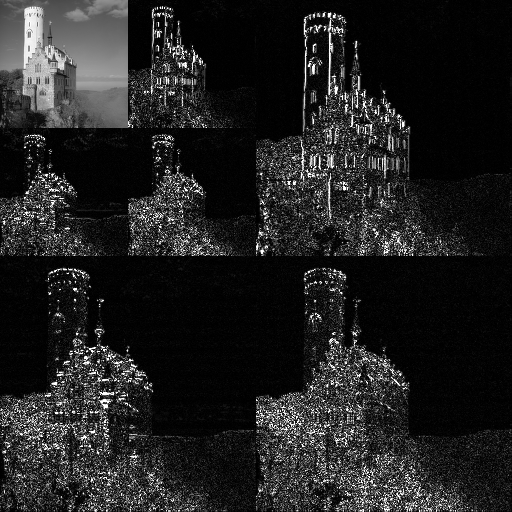
\includegraphics[width=.7\textwidth]{doc/thesis/0_figures/jp2_jpeg/Jpeg2000_2-level_wavelet_transform-lichtenstein.png}
        \caption{Hierarchical structure of an image transformed with 2-level \gls{dwt} \cite{Commons2019File:Jpeg2000Repository}.}
        \label{fig:jp2_hierarchy}
\end{figure}

A comparison of an image compressed with \gls{jpeg} and with \gls{jp2} with roughly similar compression ratio is shown in Figure~\ref{fig:jpg_jp2_comparison}. It is clearly visible that artefacts are created around the contours in the \gls{jpeg} image in contrast to the \gls{jp2} image, despite the higher compression ratio of the \gls{jp2} image.
\begin{figure}[htb]
    \centering
    \begin{subfigure}[b]{0.7\textwidth}
        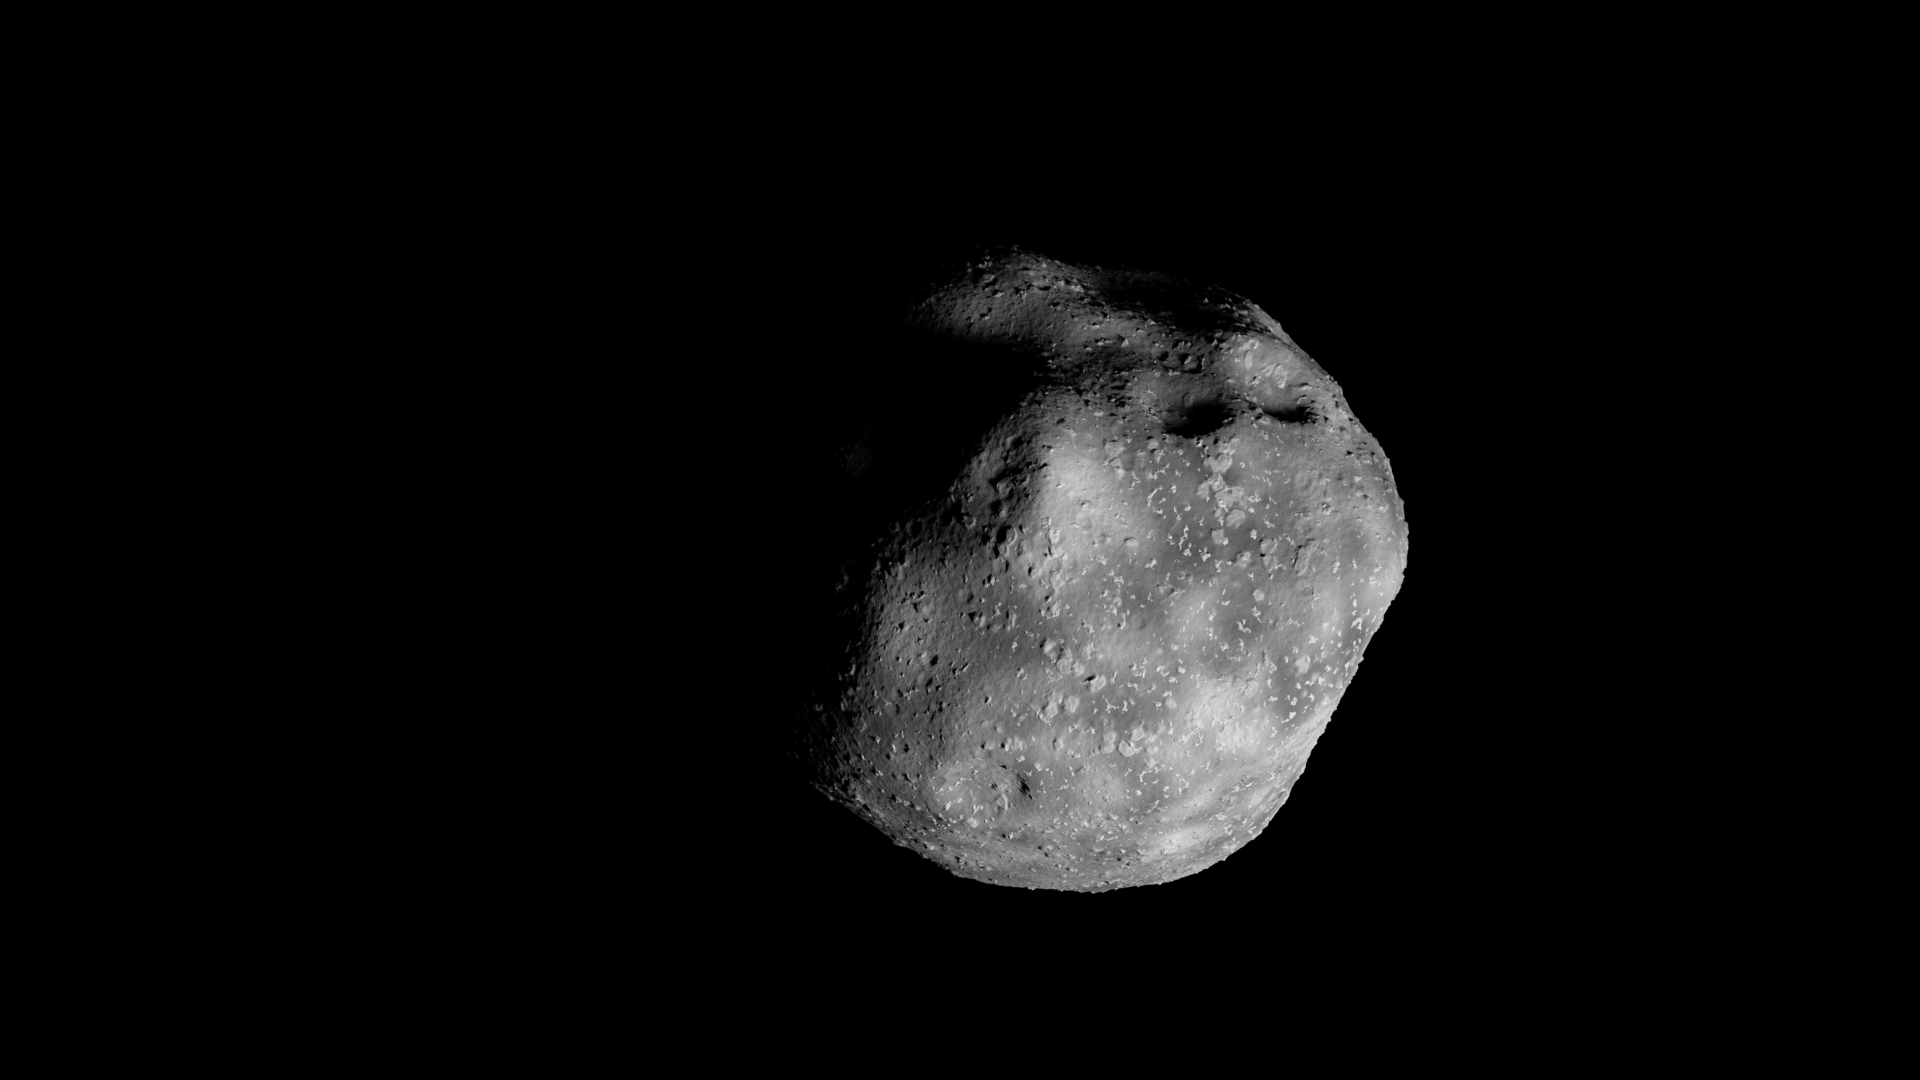
\includegraphics[width=\textwidth]{doc/thesis/0_figures/jp2_jpeg/orig.png}
        \caption{Original image without compression.}
        \label{fig:jpg_jp2_oirg}
    \end{subfigure}
    \\
    \begin{subfigure}[b]{0.48\textwidth}
        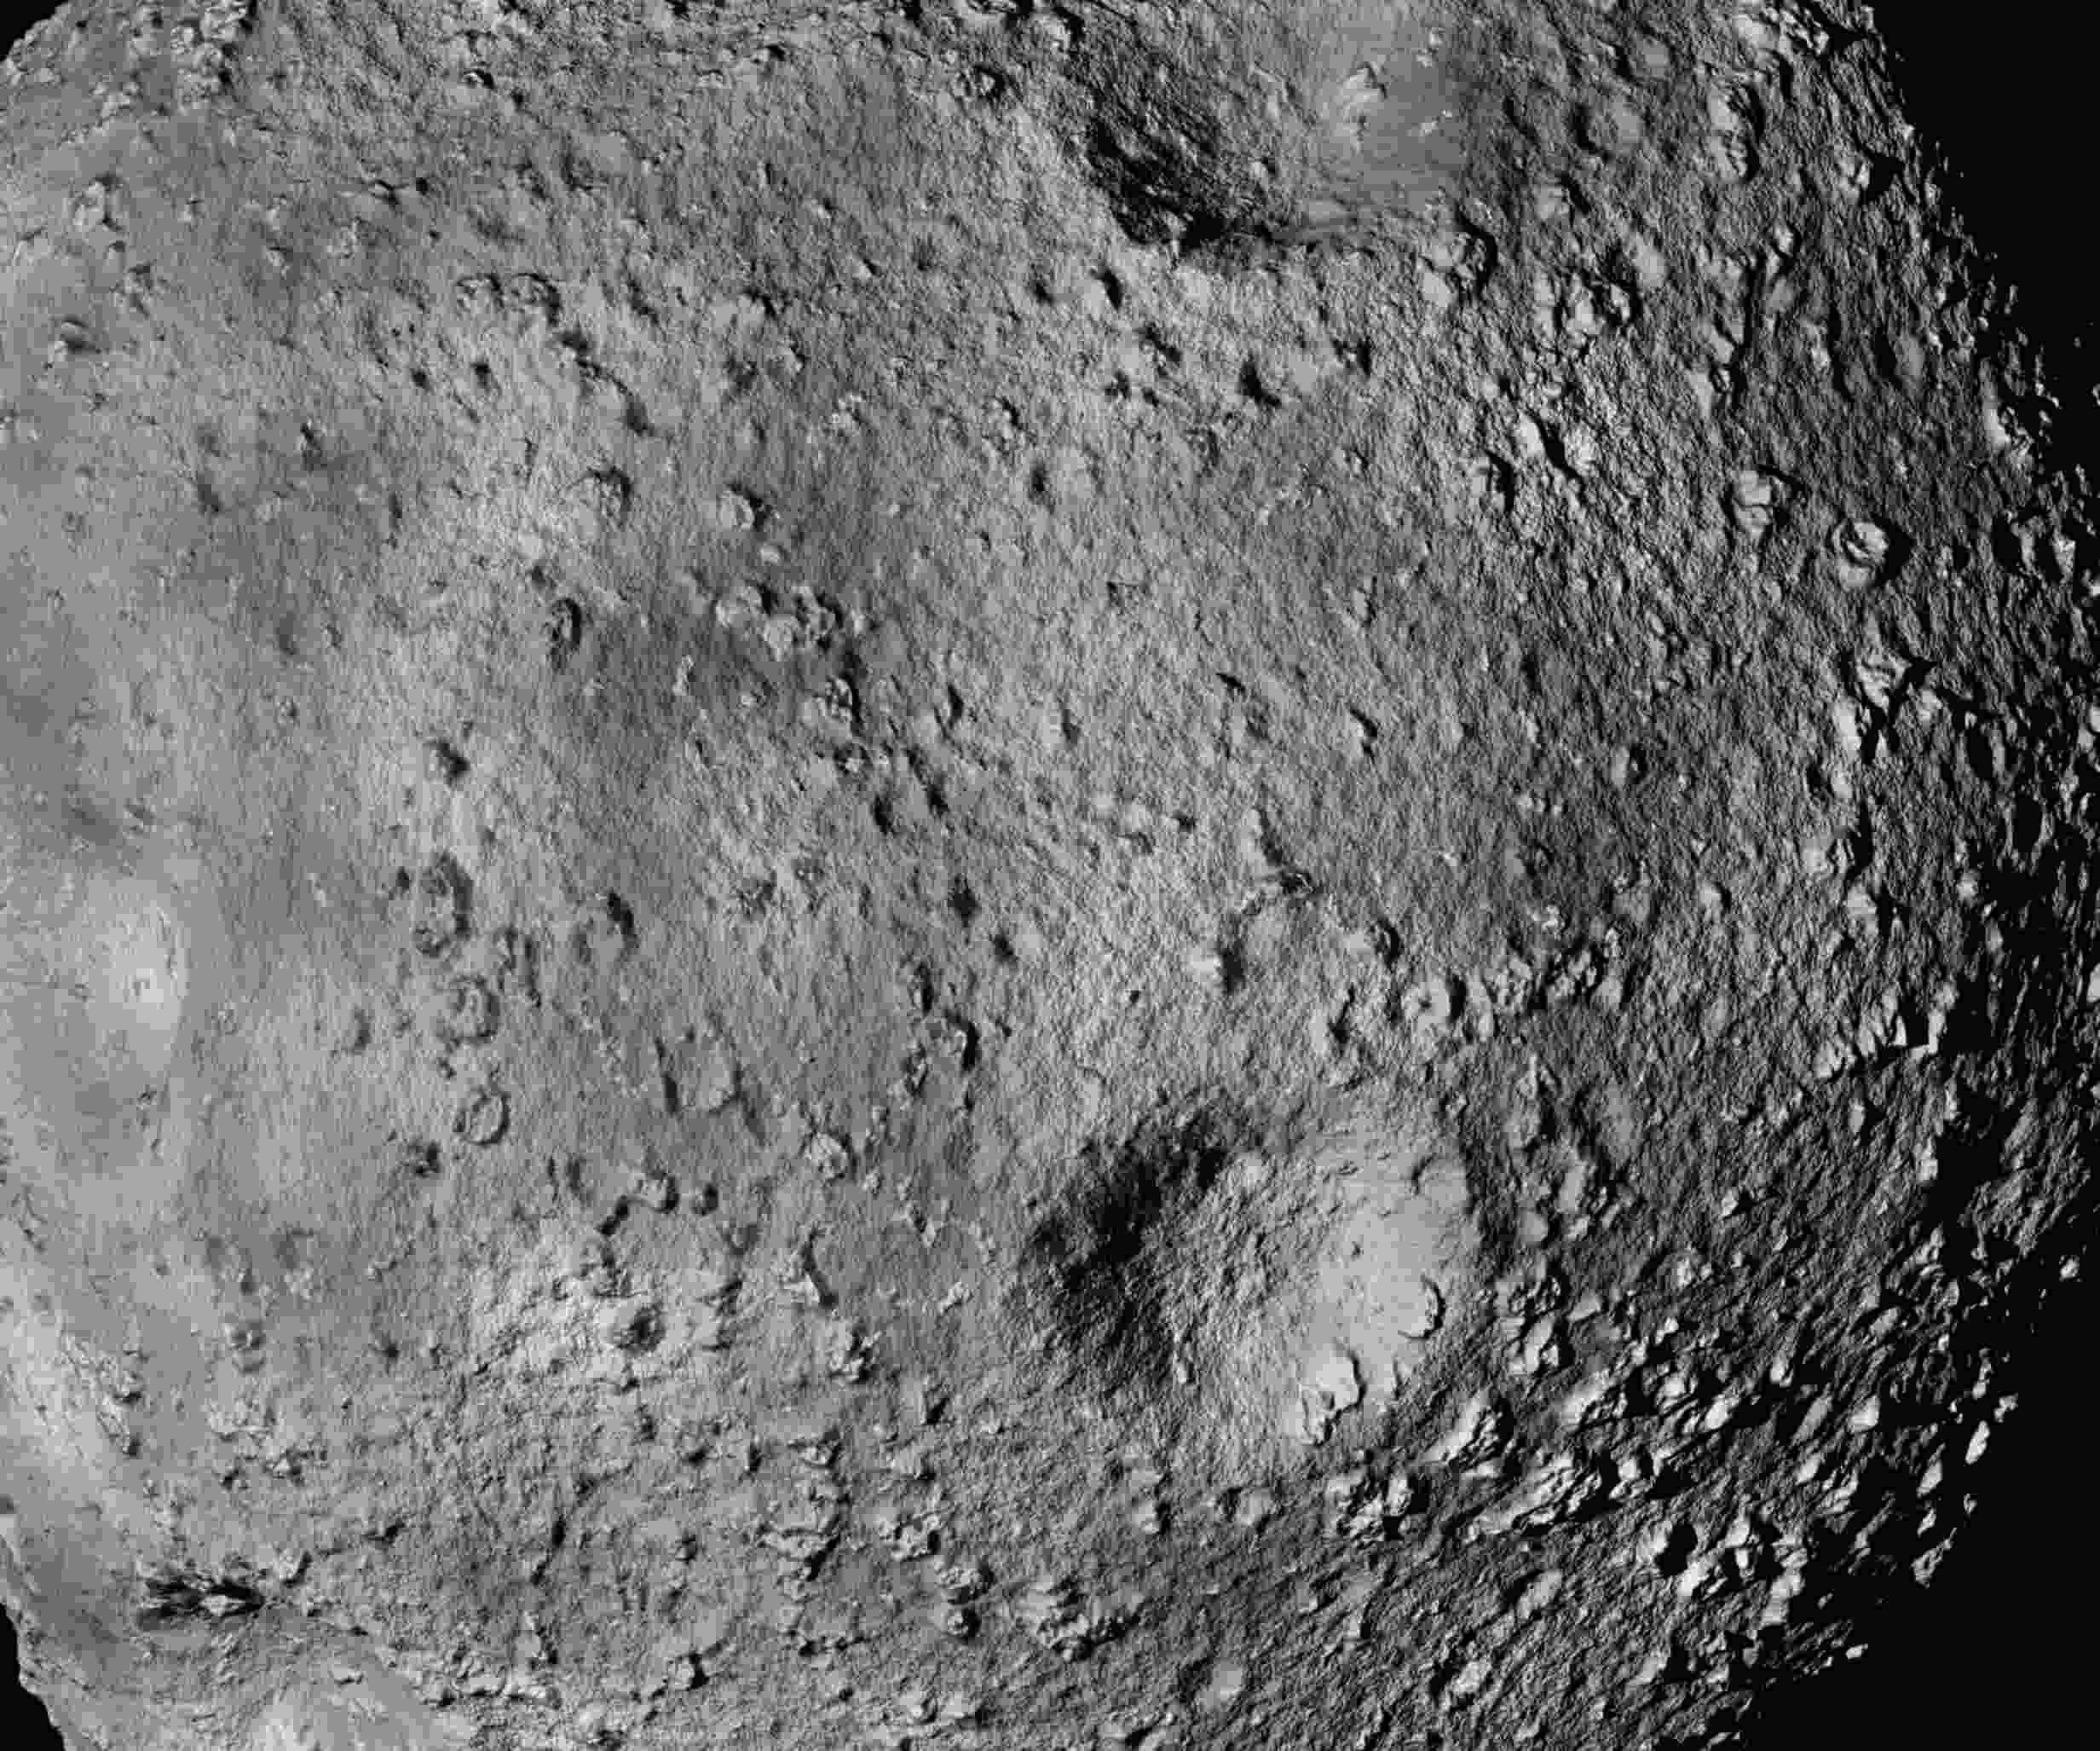
\includegraphics[width=\textwidth]{doc/thesis/0_figures/jp2_jpeg/proc_5.jpg}
        \caption{}
        \label{fig:jpg_jp2_jpeg}
    \end{subfigure}
    \begin{subfigure}[b]{0.48\textwidth}
        \includegraphics[width=\textwidth]{doc/thesis/0_figures/jp2_jpeg/proc_11.png}
        \caption{}
        \label{fig:jpg_jp2_jp2}
    \end{subfigure}
    \caption{Comparison of compression images compressed with different algorithms. Despite having a higher compression ratio, the \gls{jp2} image produces a better result for a \gls{sssb} image. (a) Raw image without compression. (b) Image compressed with \gls{dct} using the \gls{jpeg} format with a compression ratio of 61.2:1. (c) Image compressed with \gls{dwt} using the \gls{jp2} format with a compression ratio of 64.3:1.}
    \label{fig:jpg_jp2_comparison}
\end{figure}

\subsubsection{Gaussian Filtering} \label{sec:t_gauss}
Gaussian Filtering refers to convolving an image with the \gls{2d} Gaussian function. It is used to blur images and remove noise. The \gls{2d} Gaussian function with a mean of zero is defined as
\begin{align}
    G(x,y) = \frac{1}{2\pi \sigma^{2}}e^{-\frac{x^2+y^2}{2\sigma^2}}, \label{eq:gauss_2d}
\end{align}
where $\sigma$ is the standard deviation of the Gaussian distribution, and $x$ and $y$ are the coordinates.
In its theoretical version, the Gaussian distribution would extend to infinity. To be practically applied in a digital system, the Gaussian distribution needs to be cut at a certain distance from the centre. The range over which the filter is applied is the kernel size which is normally related to its standard deviation, since \SI{99}{\percent} of the distribution falls within 3 standard deviations. In addition, the Gaussian distribution needs to be discretised to be usable in a digital system. The \gls{2d} Gaussian filter is rotationally symmetric and larger standard deviation result in more blurring due to a wider peak.

\subsubsection{Down-sampling with Local Means} \label{sec:t_downsample}
Down-sampling is the process of reducing the number of pixels in an image. When down-sampled with local means, it refers to taking the average of a small set of pixels and using it as the new value of a single pixel. For example, if an image shall be reduced by a factor of two, the value of four pixels of the input are averaged for a single pixel of the output. In the example below a $4\times4$ matrix is down-sampled by a scaling factor of two to give a $2\times2$ matrix.
\begin{align*}
    \begin{bmatrix}
        1  & 2  & 3  & 4\\
        5  & 6  & 7  & 8\\
        9  & 10 & 11 & 12\\
        13 & 14 & 15 & 16\\
    \end{bmatrix} 
    \rightarrow 
    \begin{bmatrix}
        3.5  & 5.5\\
        11.5 & 13.5\\ 
    \end{bmatrix}
\end{align*}
